\section{C-Reducibility}
\label{sec:creduce}

The original proof of the four color theorem used an unavoidable set of C or D reducible configurations. C-reducibility can be thought of as a stronger but more complicated form of D-reducibility. In 2009, John P. Steinberger gave an unavoidable set of D-reducible configurations. With this, C-reducibility is no longer required to prove the four color theorem. However, the concept of C-reducibility is still insightful. Therefore we explain it here.

\subsection{Definitions}

Recall that D-reducibility required that all possible ring colorings $\Phi(n)$ are in the implying set $\overline{\Phi}(C)$. If a configuration is not D-reducible, then there must be ring colorings in $\Phi(n)$ that are not in $\overline{\Phi}(C)$. These colorings can not be converted to coloring of $C$ by flipping Kempe-chains. It is these colorings that we want to avoid with C-reducibility. By replacing $C$ with a reducer $(S,\sigma)$ consisting of a smaller graph $S$ and a ring contraction $\sigma$ we can avoid these colorings. For this to happen, the un-contracted ring colorings of $(S,\sigma)$ denoted by $\Phi(S, \sigma)$ must be in $\overline{\Phi}(C)$.

\begin{figure}[!h]
    \centering
    \begin{tikzpicture}[scale=1.0]
        \draw (0, 0) ellipse (3cm and 1.8cm);
        \draw (0, -0.3) ellipse (2cm and 1.2cm);
        \draw[fill opacity=0.4, pattern=north east lines] (0.8, -0.6) ellipse (0.8cm and 0.6cm);
        \draw[dotted, thick] (-0.7, -0.4) ellipse (1.0cm and 0.6cm);

        \node at (0.9, -0.6) { $\Phi_0(C)$ };
        \node at (0.3, 0.35) { $\overline{\Phi}(C)$ };
        \node at (0, 1.35) { $\Phi(n)$ };
        \node at (-0.8, -0.4) { $\Phi(S, \sigma)$ };
    \end{tikzpicture}

    \caption{C-reducibility requires that for some choice of a reducer $(S,\sigma)$, the colorings $\Phi(S, \sigma)$ can be converted to valid ring colorings of $C$ in $\Phi_0(C)$.}
    \label{fig:cred}
\end{figure}

Therefore, C-reducibility can be seen as an extension of D-reducibility with the reducer $(S, \sigma)$ acting as a "filter" of ring colorings. This way we can ignore those ring colorings that are not in $\overline{\Phi}(C)$. As can be seen in Figure \ref{fig:cred}, there are still colorings for the ring that are not in $\overline{\Phi}(C)$. However, we avoid them using the colorings of the reducer $\Phi(S, \sigma)$.

Let us start with the definition of a ring contraction.

\begin{definition}
    A ring contraction $\sigma(v)$ is a map from the vertices of a ring $R$ to the contracted ring $\sigma \circ R$. We require
    
    \begin{itemize}
        \item The contracted ring $\sigma \circ R$ is a valid planar graph.
        \item Neighboring ring vertices $v_i$ and $v_{i+1}$ are not contracted.
    \end{itemize}
\end{definition}

Ring contractions allows the reducer to shrink the number of boundary vertices. This simplifies the coloring problem for the reducer. Without a ring contraction, our reducer would still have the same ring as our configuration $C$, making it equally difficult to work with. Why do we not simply delete vertices from the ring of $C$? The contraction defines a map that allows us to convert boundary colorings of $(S,\sigma)$ to ring colorings of $C$ simply by un-contracting. 

\begin{figure}[!h]
    \centering
    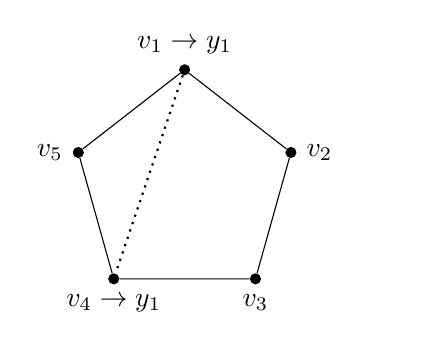
\begin{tikzpicture}[scale=1.5]
        \node[circle, fill, scale=0.015cm, label=above:{$v_1 \rightarrow y_1$}] (l1) at (0, 1) { };
        \node[circle, fill, scale=0.015cm, label=right:{$v_2$}] (l2) at (0.9, 0.30) { };
        \node[circle, fill, scale=0.015cm, label=below:{$v_3$}] (l3) at (0.6, -0.77) {};
        \node[circle, fill, scale=0.015cm, label=below:{$v_4 \rightarrow y_1$}] (l4) at (-0.6, -0.77) {};
        \node[circle, fill, scale=0.015cm, label=left:{$v_5$}] (l5) at (-0.9, 0.30) {};
        \draw (l1) -- (l2) -- (l3) -- (l4) -- (l5) -- (l1);
        \draw[dotted, thick] (l1) -- (l4);
        \node at (1.7, -0.2) { $\implies$ };
    \end{tikzpicture}
    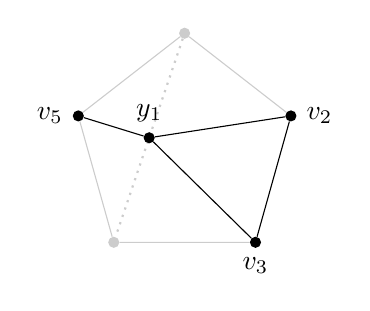
\begin{tikzpicture}[scale=1.5]
        \node[circle, fill, opacity=0.2, scale=0.015cm] (l1) at (0, 1) {};
        \node[circle, fill, opacity=0.2, scale=0.015cm] (l4) at (-0.6, -0.77) {};
        \node[circle, fill, scale=0.015cm, label=above:{$y_1$}] (y1) at (-0.3, 0.115) {};

        \node[circle, fill, scale=0.015cm, label=right:{$v_2$}] (l2) at (0.9, 0.30) { };
        \node[circle, fill, scale=0.015cm, label=below:{$v_3$}] (l3) at (0.6, -0.77) {};
        \node[circle, fill, scale=0.015cm, label=left:{$v_5$}] (l5) at (-0.9, 0.30) {};

        \draw (l5) -- (y1) -- (l2) -- (l3) -- (y1);
        \draw[dotted, thick, opacity=0.2] (l1) -- (l4);
        \draw[opacity=0.2] (l5) -- (l1) -- (l2);
        \draw[opacity=0.2] (l3) -- (l4) -- (l5);
    \end{tikzpicture}
    \caption{A contraction on $R_5$. The two vertices $v_1$ and $v_4$ are mapped to the same vertex $y_1$, and hence get contracted together. }
    \label{fig:contract}
\end{figure}

Figure \ref{fig:contract} shows the contraction process on $R_5$. Intuitively, you should think of a contraction as the merging of pairs of vertices to a single point. However, mathematically, it is easier to work with a mapping function $\sigma$ instead. Suppose we are given a coloring $x(v)$ of a contracted ring $\sigma \circ R$. Then the composition $x \circ \sigma(v)$ is a valid coloring for $R$. This is shown in Figure \ref{fig:contractcolor}

\begin{figure}[!h]
    \centering
    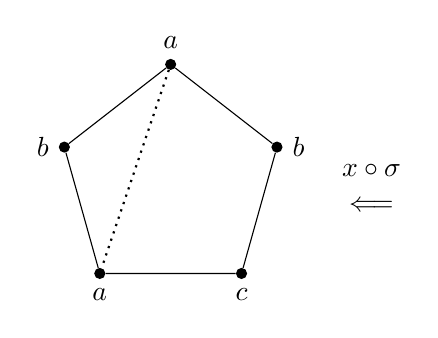
\begin{tikzpicture}[scale=1.5]
        \node[circle, fill, scale=0.015cm, label=above:{$a$}] (l1) at (0, 1) { };
        \node[circle, fill, scale=0.015cm, label=right:{$b$}] (l2) at (0.9, 0.30) { };
        \node[circle, fill, scale=0.015cm, label=below:{$c$}] (l3) at (0.6, -0.77) {};
        \node[circle, fill, scale=0.015cm, label=below:{$a$}] (l4) at (-0.6, -0.77) {};
        \node[circle, fill, scale=0.015cm, label=left:{$b$}] (l5) at (-0.9, 0.30) {};
        \draw (l1) -- (l2) -- (l3) -- (l4) -- (l5) -- (l1);
        \draw[dotted, thick] (l1) -- (l4);
        
        \node at (1.7, 0.1) { $x \circ \sigma$ };
        \node at (1.7, -0.2) { $\Longleftarrow$ };
    \end{tikzpicture}
    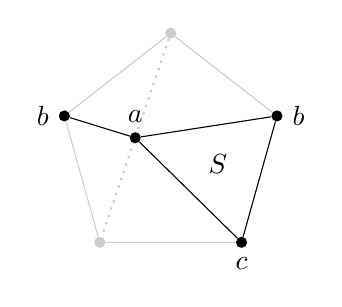
\begin{tikzpicture}[scale=1.5]
        \node[circle, fill, opacity=0.2, scale=0.015cm] (l1) at (0, 1) {};
        \node[circle, fill, opacity=0.2, scale=0.015cm] (l4) at (-0.6, -0.77) {};
        \node[circle, fill, scale=0.015cm, label=above:{$a$}] (y1) at (-0.3, 0.115) {};

        \node[circle, fill, scale=0.015cm, label=right:{$b$}] (l2) at (0.9, 0.30) { };
        \node[circle, fill, scale=0.015cm, label=below:{$c$}] (l3) at (0.6, -0.77) {};
        \node[circle, fill, scale=0.015cm, label=left:{$b$}] (l5) at (-0.9, 0.30) {};

        \draw (l5) -- (y1) -- (l2) -- (l3) -- (y1);
        \draw[dotted, thick, opacity=0.2] (l1) -- (l4);
        \draw[opacity=0.2] (l5) -- (l1) -- (l2);
        \draw[opacity=0.2] (l3) -- (l4) -- (l5);

        \node at (0.4, -0.11) { $S$ };
    \end{tikzpicture}
    \caption{ The coloring $x(v)$ of a contracted ring $\sigma \circ R$ can be converted to a coloring for the original ring $R$ using $x \circ \sigma(v)$. }
    \label{fig:contractcolor}
\end{figure}

By introducing ring contractions, we have already covered the most significant part of a reducer. The last part is the extra graph $S$ that defines the interior of our contracted ring. This extra graph $S$ is similar to the auxiliary graph $A$ that we used during the 1-reducibility proof of $R_5$. The boundary vertices of $S$ must be the same as the contracted ring $\sigma \circ R$. Now we have all the parts needed to define a reducer.

\begin{definition}
    A reducer of a configuration $C$ is a pair $(S, \sigma)$  consisting of a ring contraction $\sigma$ and a graph $S$ on less vertices than $C$ that has a boundary equal to the contracted ring $\sigma \circ R$.
\end{definition}

Of course, every reducer will reduce the size of a configuration $C$. However, for actual reducibility, we can not simply take any reducer. Our reducer $(S, \sigma)$ must satisfy the filtering property mentioned at the beginning of this section. That is, its ring colorings $\Phi(S, \sigma)$ must be contained in $\overline{\Phi}(C)$. Let us define this set.

\begin{definition}
    Let $(S, \sigma)$ be a reducer. The set of un-contracted ring colorings $\Phi(S, \sigma)$ consists of all the colorings $x \circ \sigma$ with $x(v)$ a boundary coloring of $S$.
\end{definition}

Following this definition, C-reducibility is a simple concept.

\begin{definition}
    A configuration $C$ is C-reducible if $\Phi(S,\sigma) \subset \overline{\Phi}(C)$ for some reducer $(S,\sigma)$.
\end{definition}

Now suppose we have a graph $G$ where $C$ is an embedded C-reducible configuration with reducer $(S,\sigma)$. Suppose that two non-neighboring ring vertices of $C$ are connected by an edge in $G$. If we would contract these vertices together, then we would create a loop on the boundary of $S$. We can not color vertices with loops without breaking the rules of a coloring. Therefore, we must take care to avoid such loops.

Since this issue is specific to the way the configuration $C$ is embedded in the graph $G$, we will give a name to the type of embedding that we are after.

\begin{definition}
    A configuration $C$ is $\sigma$-properly embedded in $G$ if two ring vertices of $C$ that are connected by an non-ring edge in $G$ are not contracted by $\sigma(v)$.
\end{definition}

\begin{definition}
    The C-reducible configuration $C$ has a safe reducer  $(S,\sigma)$ if it only occurs $\sigma$-properly embedded in a Birkhoff graph.
\end{definition}

Before we can use C-reducible configurations to reduce counterexamples, we must first prove the existence of a safe reducer. This was a major source of complications in the original proof of the four color theorem by Appel and Haken. This is a strong condition on the structure of a reducer. We will see examples of safe and unsafe reducers in the next section.

\subsection{C-Reducibility of the Birkhoff diamond}
\label{sec:diamond}

Although we have already shown that the Birkhoff diamond is D-reducible, we will use it as a slightly more interesting example of C-reducibility. A reducer for the Birkhoff diamond we have picture below.

\begin{figure}[!h]
    \centering
    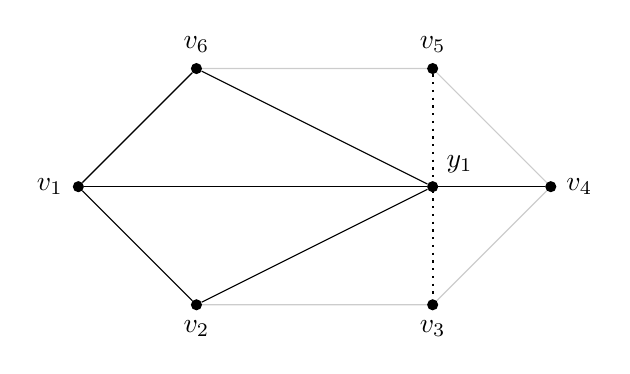
\begin{tikzpicture}[scale=1.5]
        \node[circle, fill, scale=0.015cm, label=left:$v_1$] (l1) at (-2, 0) { };
        \node[circle, fill, scale=0.015cm, label=above:$v_6$] (l2) at (-1, 1) { };
        \node[circle, fill, scale=0.015cm, label=below:$v_2$] (l4) at (-1, -1) {};

        \node[circle, fill, scale=0.015cm,label=right:$v_4$] (r1) at (2, 0) {};
        \node[circle, fill, scale=0.015cm,label=above:$v_5$] (r2) at (1, 1) {};
        \node[circle, fill, scale=0.015cm,label=below:$v_3$] (r4) at (1, -1) {};

        \node[circle, fill, scale=0.015cm,label=above right:$y_1$] (y1) at (1, 0) {};

        \draw[opacity=0.2] (l1) -- (l2) -- (r2) -- (r1) -- (r4) -- (l4) -- (l1);
        \draw[dotted, thick] (r2) -- (r4);
        \draw (l1) -- (l2) -- (y1) -- (l4) -- (l1);
        \draw (l1) -- (y1) -- (r1);
    \end{tikzpicture}
    \caption{A reducer for the Birkhoff diamond (in bold) with a single contraction on $v_4$ and $v_2$, and a single edge added by $S$. }.
    \label{fig:diamondreducer}
\end{figure}

Let us now prove the C-reducibility of the Birkhoff diamond with this reducer. First, we determine the set of colorings that the reducer creates for the original ring $R_6$.

\begin{equation}
    \Phi(S, \sigma) = \left\{ \begin{matrix}
        ababcd, & abcbdc, & abcbcd, \\ abcbac, & abcbad, & \underline{ababac}
    \end{matrix}\right\}
\end{equation}

By looking at Table \